%%%%%%%%%%%
% RESULTS %
%%%%%%%%%%%

\section{Experimental Results and Discussion}

In this section, we present and discuss our results for CIFAR-10/ViT and MNIST/CNN. 
%%%%%%%%%%%%%%%%%%%%%%%%%%%%%%%%%%%%%
% CIFAR10 MNIST SOFTMAX DISTANCE TO %
% CLUSTER CENTROID STATISTICS       %
%%%%%%%%%%%%%%%%%%%%%%%%%%%%%%%%%%%%%

\begin{table*}[ht]
\centering
\begin{tabular}{c|cccccc|cccccc}
\hline
& \multicolumn{6}{c|}{Training Dataset Correct Predictions} & \multicolumn{6}{c}{Training Dataset Incorrect Predictions} \\
Digit & Mean & Median & Min & Max & $\sigma$ & Count & Mean & Median & Min & Max & $\sigma$ & Count \\ \hline
0 & 0.0166 & 0.0088 & 0.0018 & \textbf{0.8433} & 0.0536 & 5890 & 0.9955 & 0.9552 & \textbf{0.7037} & 1.3681 & 0.1756 & 33 \\
1 & 0.0154 & 0.0085 & 0.0020 & \textbf{0.7051} & 0.0486 & 6704 & 1.0912 & 1.0771 & \textbf{0.7247} & 1.3909 & 0.2197 & 38 \\
2 & 0.0370 & 0.0208 & 0.0056 & \textbf{0.7453} & 0.0746 & 5859 & 1.0409 & 1.0460 & \textbf{0.6962} & 1.3912 & 0.2064 & 99 \\
3 & 0.0352 & 0.0192 & 0.0055 & \textbf{0.7509} & 0.0754 & 6019 & 1.0522 & 1.0338 & \textbf{0.7139} & 1.3999 & 0.2143 & 112 \\
4 & 0.0295 & 0.0166 & 0.0031 & \textbf{0.6933} & 0.0661 & 5755 & 1.0681 & 1.0642 & \textbf{0.7139} & 1.4010 & 0.2045 & 87 \\
5 & 0.0298 & 0.0165 & 0.0024 & \textbf{0.7634} & 0.0693 & 5339 & 1.0572 & 1.0560 & \textbf{0.7066} & 1.3956 & 0.2000 & 82 \\
6 & 0.0154 & 0.0081 & 0.0015 & \textbf{0.7981} & 0.0485 & 5884 & 1.0485 & 1.0702 & \textbf{0.7068} & 1.4015 & 0.2110 & 34 \\
7 & 0.0302 & 0.0171 & 0.0028 & \textbf{0.7365} & 0.0678 & 6199 & 1.0133 & 0.9764 & \textbf{0.6960} & 1.3989 & 0.2160 & 66 \\
8 & 0.0619 & 0.0363 & 0.0092 & \textbf{0.7788} & 0.0989 & 5581 & 1.0232 & 1.0083 & \textbf{0.6852} & 1.3816 & 0.1990 & 270 \\
9 & 0.0399 & 0.0232 & 0.0048 & \textbf{0.7616} & 0.0781 & 5844 & 1.0576 & 1.0830 & \textbf{0.7179} & 1.3974 & 0.2201 & 105 \\ \hline
& \multicolumn{6}{c|}{Testing Dataset Correct Predictions} & \multicolumn{6}{c}{Testing Dataset Incorrect Predictions} \\
Digit & Mean & Median & Min & Max & $\sigma$ & Count & Mean & Median & Min & Max & $\sigma$ & Count \\ \hline
0 & 0.0141 & 0.0075 & 0.0021 & \textbf{0.7225} & 0.0506 & 977 & 1.0329 & 1.0185 & \textbf{0.7923} & 1.2880 & 0.2026 & 3 \\
1 & 0.0126 & 0.0071 & 0.0023 & \textbf{0.6737} & 0.0445 & 1129 & 0.9823 & 0.9556 & \textbf{0.7278} & 1.2445 & 0.1898 & 6 \\
2 & 0.0354 & 0.0202 & 0.0037 & \textbf{0.6697} & 0.0704 & 1015 & 1.0855 & 1.0725 & \textbf{0.7010} & 1.3833 & 0.1844 & 17 \\
3 & 0.0331 & 0.0177 & 0.0049 & \textbf{0.7515} & 0.0765 & 998 & 0.9823 & 0.9752 & \textbf{0.7102} & 1.3230 & 0.2044 & 12 \\
4 & 0.0306 & 0.0169 & 0.0047 & \textbf{0.6603} & 0.0678 & 972 & 0.9309 & 0.8725 & \textbf{0.7073} & 1.3110 & 0.1923 & 10 \\
5 & 0.0313 & 0.0173 & 0.0051 & \textbf{0.6324} & 0.0692 & 883 & 1.1874 & 1.2976 & \textbf{0.8477} & 1.3982 & 0.2067 & 9 \\
6 & 0.0172 & 0.0088 & 0.0029 & \textbf{0.7135} & 0.0545 & 941 & 1.0737 & 1.0242 & \textbf{0.7240} & 1.4009 & 0.2120 & 17 \\
7 & 0.0295 & 0.0165 & 0.0036 & \textbf{0.6939} & 0.0678 & 1009 & 0.9665 & 0.8833 & \textbf{0.7148} & 1.3628 & 0.2016 & 19 \\
8 & 0.0616 & 0.0372 & 0.0114 & \textbf{0.7328} & 0.0918 & 934 & 1.0513 & 1.0399 & \textbf{0.7252} & 1.3842 & 0.2022 & 40 \\
9 & 0.0359 & 0.0206 & 0.0042 & \textbf{0.6870} & 0.0765 & 980 & 1.0502 & 1.0486 & \textbf{0.6968} & 1.3838 & 0.2197 & 29 \\ \hline
\end{tabular}
\captionsetup{justification=raggedright,singlelinecheck=false}
\caption{Statistical Summary of MNIST Softmax Output Distances to Centroids for Different Datasets and Prediction Outcomes. The centroids are obtained from Softmax outputs for correct class predictions from the training dataset.}
\label{tab:distance_to_centroid}
\end{table*}

% DATA for table above
%        Mean    Median       Min       Max  Standard Deviation  Count
% 0  0.016608  0.008843  0.001769  0.843304            0.053614   5890
% 1  0.015435  0.008516  0.002036  0.705149            0.048557   6704
% 2  0.036996  0.020828  0.005605  0.745250            0.074615   5859
% 3  0.035151  0.019205  0.005478  0.750860            0.075377   6019
% 4  0.029493  0.016613  0.003111  0.693346            0.066094   5755
% 5  0.029819  0.016509  0.002448  0.763396            0.069287   5339
% 6  0.015405  0.008078  0.001526  0.798075            0.048491   5884
% 7  0.030247  0.017138  0.002791  0.736508            0.067780   6199
% 8  0.061884  0.036283  0.009184  0.778795            0.098932   5581
% 9  0.039943  0.023188  0.004768  0.761636            0.078053   5844
%        Mean    Median       Min       Max  Standard Deviation  Count
% 0  0.995516  0.955230  0.703653  1.368133            0.175639     33
% 1  1.091157  1.077065  0.724706  1.390934            0.219724     38
% 2  1.040888  1.046023  0.696177  1.391211            0.206378     99
% 3  1.052159  1.033801  0.713948  1.399858            0.214313    112
% 4  1.068138  1.064157  0.713896  1.400997            0.204490     87
% 5  1.057245  1.055964  0.706555  1.395563            0.200003     82
% 6  1.048483  1.070162  0.706828  1.401450            0.211018     34
% 7  1.013332  0.976427  0.695997  1.398902            0.216013     66
% 8  1.023217  1.008262  0.685179  1.381630            0.199017    270
% 9  1.057626  1.082991  0.717850  1.397425            0.220102    105
%        Mean    Median       Min       Max  Standard Deviation  Count
% 0  0.014064  0.007518  0.002131  0.722502            0.050551    977
% 1  0.012627  0.007062  0.002254  0.673694            0.044504   1129
% 2  0.035369  0.020174  0.003719  0.669724            0.070428   1015
% 3  0.033119  0.017744  0.004876  0.751473            0.076455    998
% 4  0.030573  0.016858  0.004709  0.660308            0.067756    972
% 5  0.031271  0.017275  0.005053  0.632375            0.069207    883
% 6  0.017175  0.008774  0.002851  0.713528            0.054455    941
% 7  0.029476  0.016466  0.003639  0.693906            0.067756   1009
% 8  0.061609  0.037214  0.011389  0.732832            0.091848    934
% 9  0.035850  0.020602  0.004236  0.686980            0.076507    980
%        Mean    Median       Min       Max  Standard Deviation  Count
% 0  1.032918  1.018475  0.792297  1.287982            0.202620      3
% 1  0.982310  0.955644  0.727825  1.244521            0.189784      6
% 2  1.085502  1.072510  0.700976  1.383269            0.184444     17
% 3  0.982309  0.975231  0.710249  1.322951            0.204446     12
% 4  0.930852  0.872484  0.707302  1.310962            0.192325     10
% 5  1.187412  1.297633  0.847685  1.398223            0.206653      9
% 6  1.073695  1.024168  0.724028  1.400876            0.211957     17
% 7  0.966459  0.883283  0.714793  1.362762            0.201621     19
% 8  1.051282  1.039866  0.725232  1.384221            0.202232     40
% 9  1.050175  1.048609  0.696760  1.383811            0.219746     29

%\subsection{Softmax Distance to Class Centroid Statistics}
% Discussion about table results
\noindent \textbf{Softmax Distance to Class Centroid Statistics:} We store the softmax outputs, true and predicted labels for the MNIST and CIFAR-10 training datasets, we obtain the mean values for all correctly predicted classes, use the values in algorithm \ref{alg:k-means-centroid-init}  to initialise the cluster centroids, then using the procedure described in algorithm \ref{alg:min_distance} and the same hardware used to train the MNIST classifier CNN, generate K-Means clusters and compute statistics as presented in Table \ref{tab:distance_to_centroid} (for the MNIST results), a summary of the distances between the softmax outputs of a model and the centroids for each digit class (0-9) in the MNIST dataset. The centroids are calculated using the softmax outputs for correct predictions from the training dataset. The table is divided into four main sections: Training Dataset Correct Predictions, Training Dataset Incorrect Predictions, Testing Dataset Correct Predictions, and Testing Dataset Incorrect Predictions. For each digit and section, statistics are displayed with respect to softmax distance from each class to its centroid: the mean, median, minimum (highlighted in bold for the testing datasets), maximum (highlighted in bold for the training datasets), standard deviation ($\sigma$), and count of instances are provided. We note that for the correct predictions, the mean softmax distance to class centroid for digits zero, one and six are lowest (network prediction accuracy is high) while for digit 8 the mean softmax distance to class centroid is a comparatively larger value (netrowk prediction accuracy is not as high). The significance of the bold highlight for Max values in the Training section, and Min values in the Correct Prediction sections, is that the Min values in the Incorrect Predictions sections, is that the latter is effectively the Threshold we propose be used as a boundary for accepting the class prediction as accurate. Anything softmax distances equal or above the threshold will be considered not safe to use. It becomes evident by comparing both columns, that for the training dataset, there is a significant overlap between Max and Min columns, however, the testing dataset presents an interesting property in that there is less of an overlap. The significance of the overlap is that any correct predictions within the overlap will be tagged as unsafe, for the scheme we propose to hold, which means more manual classification and human intervention on the downside, and on the upside a high likelihood that every prediction with softmax distance below the threshold is accurate.

In practice a small number of samples, 0.04\%, consistent across both CIFAR-10 and MNIST testing dataset prediction, are found in the overlap, as shown later in Tables \ref{tab:centroid_distance_overlap_mnist} and \ref{tab:centroid_distance_overlap}. Also shown in Table \ref{tab:distance_to_centroid} are the softmax distance standard deviations and counts for correct and incorrect classifications.

%\subsection{Predictive Accuracy and Softmax Distance to Class Centroid}

\noindent \textbf{Predictive Accuracy and Softmax Distance to Class Centroid:} The confusion matrices in Figure \ref{fig:mnist_training_confusion_matrix} provide some insights into what are the most likely MNIST misclassifications at training time. We note that number zero is the digit less likely, and number eight is the digit most likely to be misclassified. Other digits that are less likely to be misclassified are digits one and; six in the training dataset, and five in the testing dataset. Digit eight is likely to be misclassified as six or nine, while digit three is likely to be misclassified as two, five or nine.

%%%%%%%%%%%%%%%%%%%%%%%%%%
% MNIST CONFUSION MATRIX %
%%%%%%%%%%%%%%%%%%%%%%%%%%

% plot produced with function call:
% conf_matrix1, conf_matrix2 = display_misclassifications_side_by_side_cifar10(train_np, test_np, 10, 11, class_labels, 20, 7, True)
% \begin{figure}[ht]
%     \centering
%     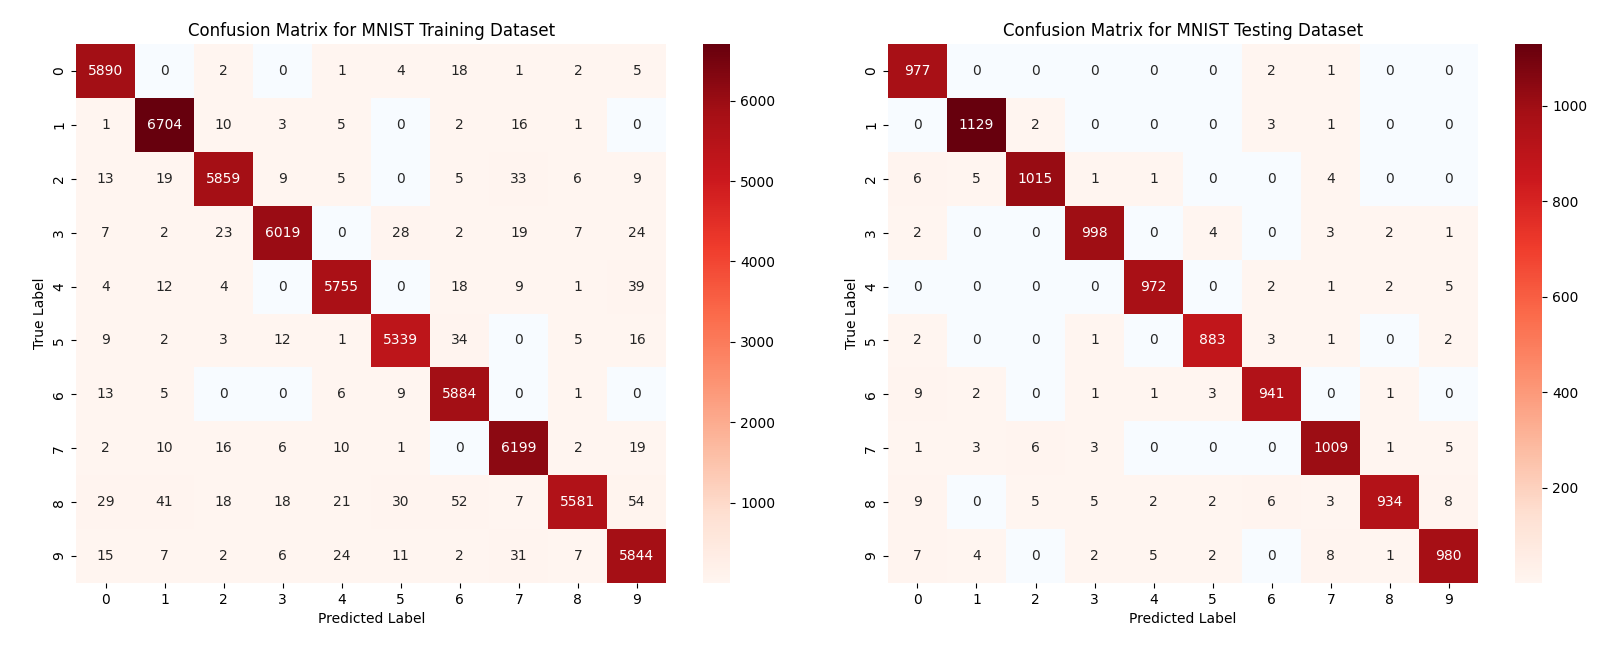
\includegraphics[width=0.99\columnwidth]{Figures/mnist_combined_confusion_matrix.png}
%     \caption{Please zoom in for detail. Confusion matrices for the MNIST classification model on the training dataset (left) and testing dataset (right). The matrices display the true labels on the vertical axis and the predicted labels on the horizontal axis. The diagonal elements represent correctly classified instances, while the off-diagonal elements indicate misclassifications.}
%     \label{fig:mnist_combined_confusion_matrix}
% \end{figure}

\begin{figure}[ht]
    \centering
    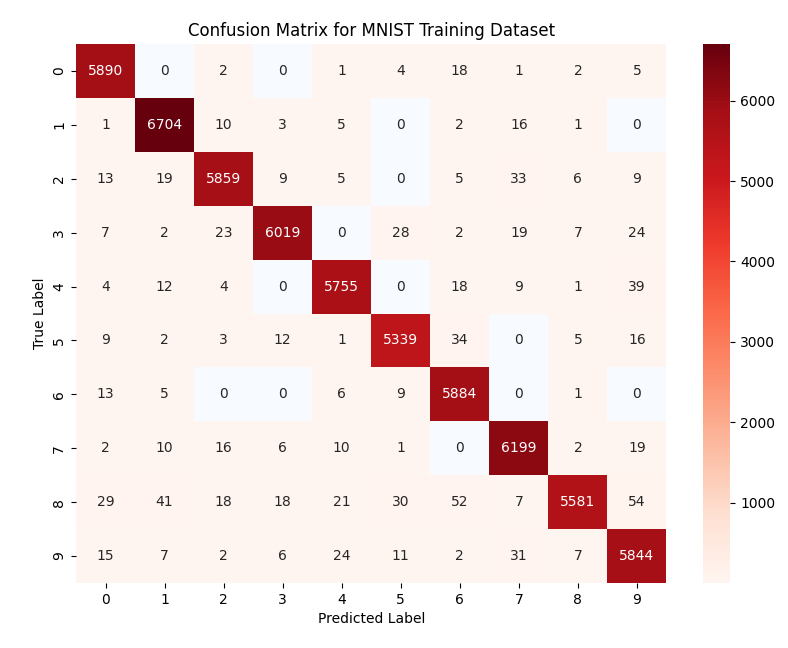
\includegraphics[width=0.99\columnwidth]{Figures/mnist_training_confusion_matrix.png}
    \caption{Confusion matrices for the MNIST classification model on the training dataset. The matrices display the true labels on the vertical axis and the predicted labels on the horizontal axis. The diagonal elements represent correctly classified instances, while the off-diagonal elements indicate misclassifications. The corresponding confusion matrix for the testing dataset is provided in the supplementary materials.}
    \label{fig:mnist_training_confusion_matrix}
\end{figure}

The confusion matrix for the CIFAR-10 training dataset in Figure \ref{fig:cifar10_training_confusion_matrix} illustrates the performance of a classifier model on the training dataset. For the training set, the model exhibits a strong diagonal, indicative of high classification accuracy for most classes. Nonetheless, certain classes show notable confusion, such as 'cat' with 'dog' and 'deer' with 'frog', and the confusion is reflected in the class softmax distance to cluster centroid.

Examining the testing dataset, the model achieves good classification success, with perfect recognition of 'frog' class. Misclassifications are present but considerably reduced compared to the training dataset, particularly for pairs such as 'truck' and 'automobile', as well as 'cat' and 'dog'. The reduced confusion in the test set is also reflected in the softmax distance to cluster centroid.

% plot produced with function call:
% conf_matrix1, conf_matrix2 = display_misclassifications_side_by_side_cifar10(train_np, test_np, 10, 11, class_labels, 20, 7, True)
\begin{figure}[ht]
    \centering   
    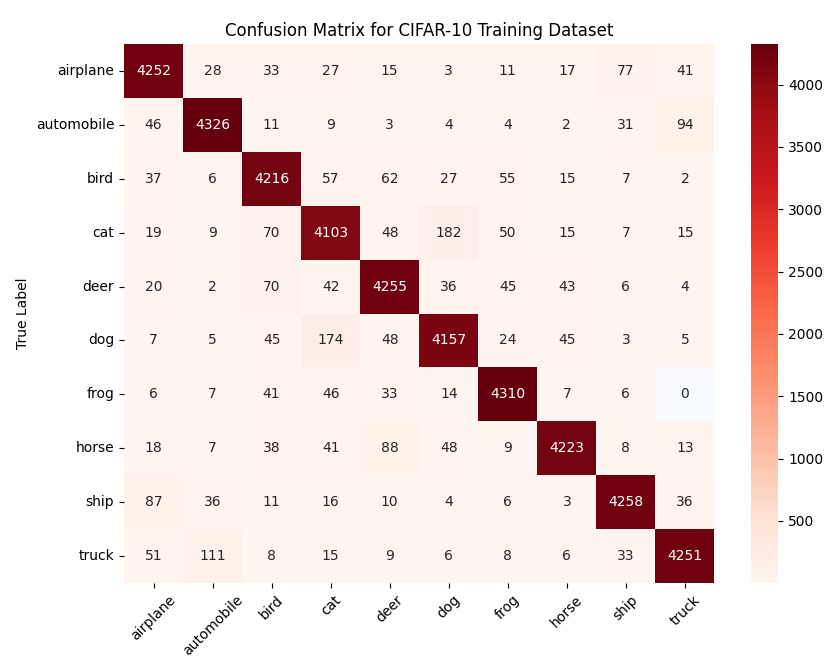
\includegraphics[width=0.99\columnwidth]{Figures/cifar10_training_confusion_matrix.png}
    \caption{Confusion matrix for the CIFAR-10 classifier model training dataset dataset dataset correct and incorrect classifications. The corresponding matrix for the testing dataset is given in the supplementary materials.}
    \label{fig:cifar10_training_confusion_matrix}
\end{figure}



%%%%%%%%%%%%%%%%%%%%%%%%%%%%%%%%%
% CIFAR10 BOXPLOTS SIDE BY SIDE %
%%%%%%%%%%%%%%%%%%%%%%%%%%%%%%%%%

%\subsection{Overlap between maximum and minimum softmax distances to class centroids}

% Figure \ref{fig:CIFAR10_boxplots_side_by_side_x2} presents box plots showing the distribution of distances to centroids for correctly and incorrectly classified instances in each class of the CIFAR-10 training and testing datasets.

% In the training dataset, the distances to centroids for correctly classified instances (green boxes) are generally lower than those for incorrectly classified instances (red boxes), indicating that correctly classified instances tend to be closer to their respective class centroids in the feature space. However, there is a small overlap between the distances of correctly and incorrectly classified instances, particularly in classes such as cat, dog, and deer. 

% The testing dataset exhibits a similar trend, with correctly classified instances having lower distances to centroids compared to incorrectly classified instances. The overlap between the two groups is less pronounced in the testing dataset, such as in classes like frog. This decreased overlap is expected, as the softmax distance to cluster centroids for incorrect classifications is larger, compared to training dataset. Note there is no frog boxplot for incorrect classifications, as reflected in the confusion matrix.

% The side-by-side boxplots convey the distributions of distances to centroids for both the training and testing sets, categorized by class. These distances are represented on a logarithmic scale, facilitating the visualization of a wide range of values. The boxplots are bifurcated into two sections for each class: correctly classified and incorrectly classified instances.

% For both the training and testing sets, there is a clear pattern where the correctly classified instances tend to have a smaller median distance to the class centroid compared to the incorrectly classified ones. This observation is consistent across all classes, suggesting that instances closer to the centroid of their respective class in the feature space are more likely to be classified correctly by the model. The notable overlap in the interquartile ranges, however, indicates that while distance to the centroid is an informative metric, it is not solely determinative of classification accuracy.

% The incorrectly classified instances exhibit greater variance in distances to the centroid, as evidenced by the longer whiskers and the presence of outliers. This variability implies that misclassified instances can sometimes be far off from the core cluster of their true class, potentially falling closer to the regions dominated by other classes in the feature space. This is indicative of boundary cases or instances that bear a resemblance to multiple categories.

% The consistency of these trends between the training and testing sets indicates that the distance to the centroid is a robust indicator of classification difficulty across the model’s application. The presence of some correctly classified instances at higher distances suggests that other factors also influence classification accuracy, such as the density of data points in the surrounding feature space, class overlap, or specific intra-class variabilities.

\noindent \textbf{Overlap between maximum and minimum softmax distances to class centroids:} Figure \ref{fig:CIFAR10_boxplots_side_by_side_x2} presents box plots showing the distribution of distances to centroids for correctly and incorrectly classified instances in each class of the CIFAR-10 training and testing datasets. In the training dataset, the distances to centroids for correctly classified instances (green boxes) are generally lower than those for incorrectly classified instances (red boxes), indicating that correctly classified instances tend to be closer to their respective class centroids in the feature space. However, there is a small overlap between the distances of correctly and incorrectly classified instances, particularly in classes such as cat, dog, and deer. The testing dataset exhibits a similar trend, with correctly classified instances having lower distances to centroids compared to incorrectly classified instances. The overlap between the two groups is less pronounced in the testing dataset, such as in classes like frog. Note there is no frog boxplot for incorrect classifications, as reflected in the confusion matrix.

% Moved to Methods to better spread out figures
% \begin{figure*}[ht]
%     \centering
%     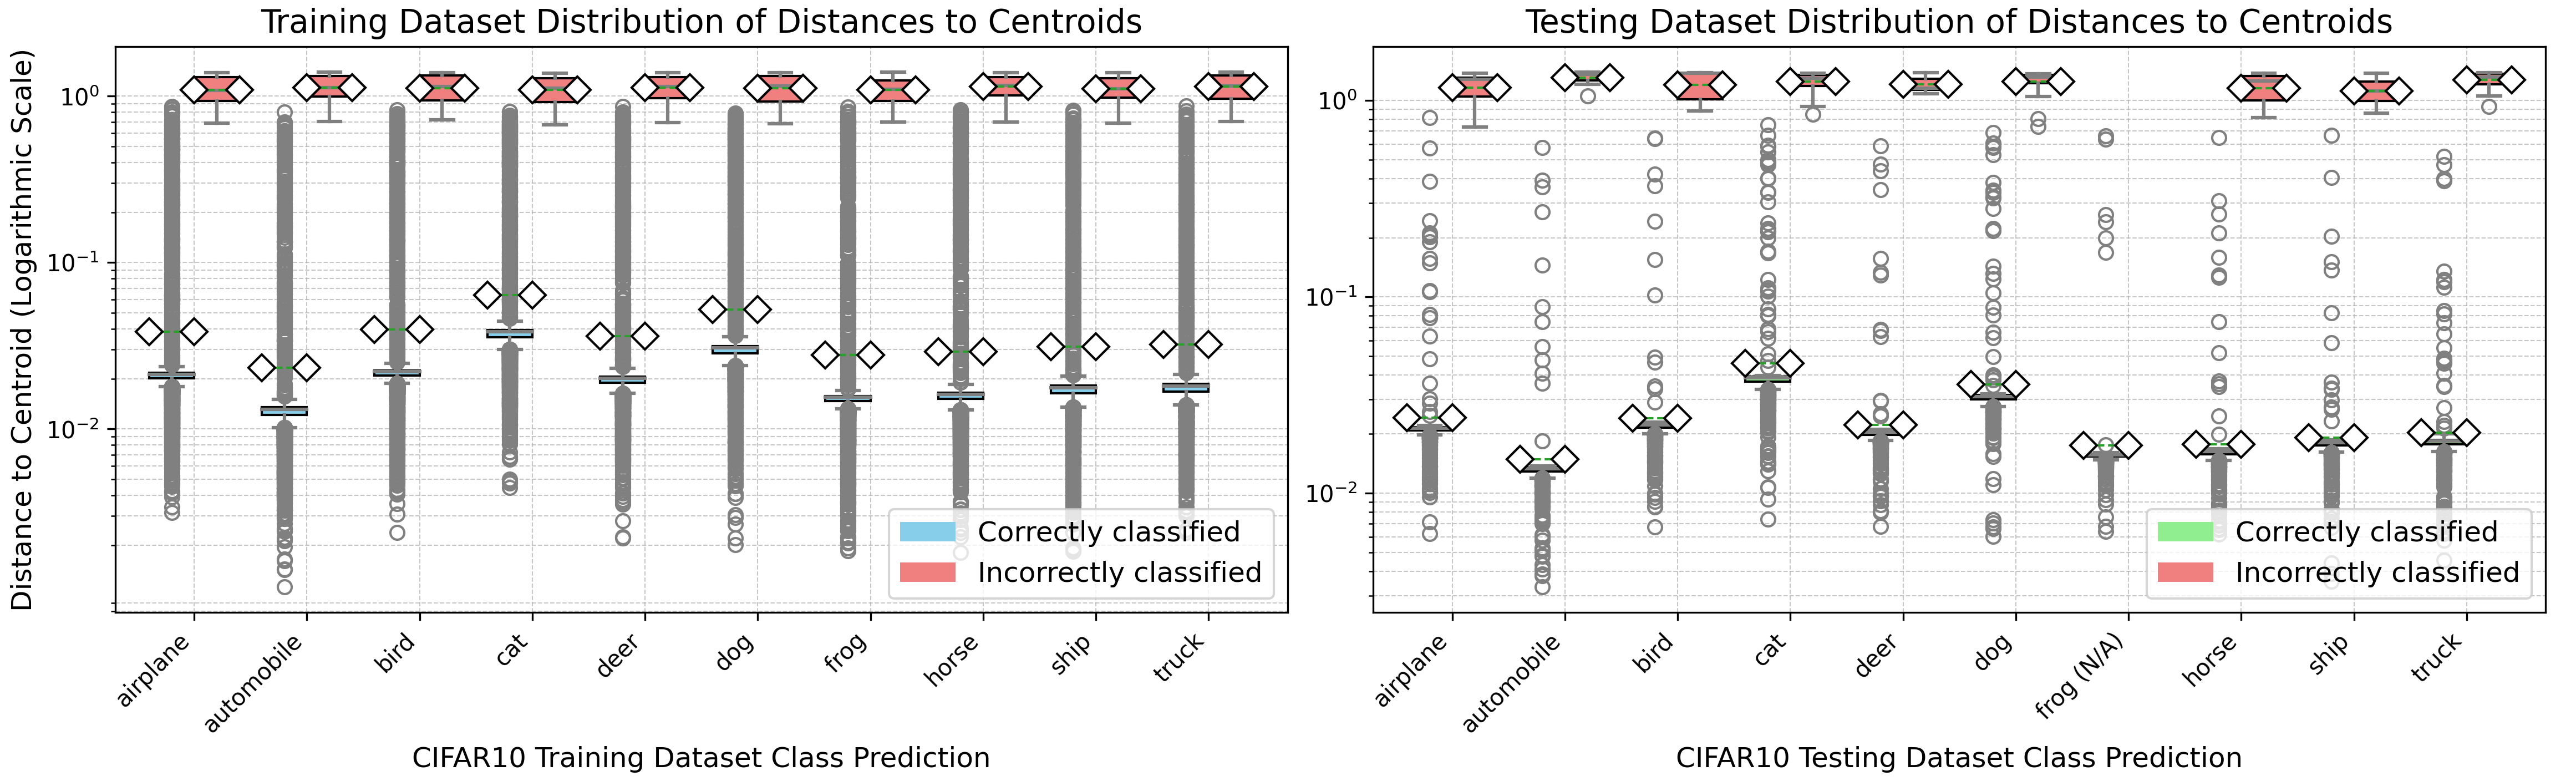
\includegraphics[width=0.99\textwidth]{Figures/CIFAR10_boxplots_side_by_side_x2.png}   \captionsetup{justification=raggedright,singlelinecheck=false}
%     \caption{Distribution of Distances to Centroids for Correctly and Incorrectly Classified Instances in Training and Testing CIFAR-10 data, where training data is on the left and testing data is displayed on the right. Distances on y axis are shown on a logarithmic scale. Centroids are obtained from correctly classified training examples, then used for both training and testing datasets, a cluster is not created from the testing softmax distances. On the testing dataset, no frogs as misclassified, hence the missing top bloxplot. The corresponding plot for the MNIST dataset results is given in the supplementary materials.}
%     \label{fig:CIFAR10_boxplots_side_by_side_x2}
% \end{figure*}

The side-by-side boxplots convey the distributions of distances to centroids for both the training and testing sets, categorized by class. These distances are represented on a logarithmic scale, facilitating the visualization of a wide range of values. For both sets, there is a clear pattern where the correctly classified instances tend to have a smaller median distance to the class centroid compared to the incorrectly classified ones. This observation is consistent across all classes, suggesting that instances closer to the centroid of their respective class in the feature space are more likely to be classified correctly by the model. The notable overlap in the interquartile ranges, however, indicates that while distance to the centroid is an informative metric, it is not solely determinative of classification accuracy.

The incorrectly classified instances exhibit greater variance in distances to the centroid, as evidenced by the longer whiskers and the presence of outliers. This variability implies that misclassified instances can sometimes be far off from the core cluster of their true class, potentially falling closer to the regions dominated by other classes in the feature space. This is indicative of boundary cases or instances that bear a resemblance to multiple categories. The consistency of these trends between the training and testing sets indicates that the distance to the centroid is a robust indicator of classification difficulty across the model's application. The presence of some correctly classified instances at higher distances suggests that other factors also influence classification accuracy, such as the density of data points in the surrounding feature space, class overlap, or specific intra-class variabilities.

% \subsection{Overlap table MNIST discussion 1}

%%%%%%%%%%%%%%%%%
% OVERLAP TABLE %
%%%%%%%%%%%%%%%%%

% Table generated with function call:
% centroid_distance_overlap_latex(d2c_train_correct, d2c_train_incorrect, d2c_test_correct, d2c_test_incorrect)
% \begin{table}[htbp]
% \centering
% \begin{tabular}{|c|c|c|c|c|c|c|}
% \hline
% Digit & \multicolumn{3}{c|}{Train Data - Train Centroids} & \multicolumn{3}{c|}{Test Data - Train Centroids} \\
% \hline
%  & Count & Total & Overlap & Count & Total & Overlap \\
% \hline
% 0 & 2 & 5890 & 0.03\% & 1 & 977 & 0.10\% \\
% 1 & 0 & 6704 & 0.00\% & 0 & 1129 & 0.00\% \\
% 2 & 1 & 5859 & 0.02\% & 0 & 1015 & 0.00\% \\
% 3 & 3 & 6019 & 0.05\% & 1 & 998 & 0.10\% \\
% 4 & 0 & 5755 & 0.00\% & 0 & 972 & 0.00\% \\
% 5 & 5 & 5339 & 0.09\% & 0 & 883 & 0.00\% \\
% 6 & 2 & 5884 & 0.03\% & 1 & 941 & 0.11\% \\
% 7 & 2 & 6199 & 0.03\% & 0 & 1009 & 0.00\% \\
% 8 & 12 & 5581 & 0.22\% & 1 & 934 & 0.11\% \\
% 9 & 1 & 5844 & 0.02\% & 0 & 980 & 0.00\% \\
% \hline
% Totals & 28 & 59074 & 0.05\% & 4 & 9838 & 0.04\% \\
% \hline
% \end{tabular}
% \caption{Counts of correctly classified training and testing image predictions with distance to centroids equal or above error threshold $\varepsilon_{\text{th}}(i)$ where $i$ is the digit class}
% \label{tab:centroid_distance_overlap_mnist}
% \end{table}

% Table \ref{tab:centroid_distance_overlap_mnist} show the counts of correctly classified training and testing examples that are assigned a  By choosing the $\varepsilon_{\text{th}}(i)$ the accuracy.

% The table presents an analysis of the counts and percentages of correctly classified images in the training and testing datasets that have softmax distances to their respective class centroids above a certain threshold. The threshold is determined by the nearest softmax distance to the centroid for the incorrectly classified classes.

% The table is divided into two main sections: "Train Data - Train Centroids" and "Test Data - Train Centroids." For each section, the table provides the count of images that satisfy the threshold condition, the total number of images in each class, and the percentage of overlap (i.e., the proportion of images above the threshold relative to the total count).

% Looking at the "Train Data - Train Centroids" section, we observe that the overlap percentages are relatively low, ranging from 0.00\% to 0.22\%. This suggests that only a small fraction of the correctly classified training images have softmax distances to their centroids above the threshold set by the incorrectly classified images. The highest overlap is observed for digit class 8, with 12 out of 5,581 images (0.22\%) having distances above the threshold.

% Similarly, in the "Test Data - Train Centroids" section, the overlap percentages are even lower, ranging from 0.00\% to 0.11\%. This indicates that the trained model is able to correctly classify the majority of the test images while maintaining a distance to the centroids below the threshold set by the incorrectly classified images. The highest overlap in the test data is observed for digit classes 6 and 8, with 1 out of 941 (0.11\%) and 1 out of 934 (0.11\%) images, respectively, having distances above the threshold.

% The "Totals" row summarizes the overall counts and overlap percentages across all digit classes. For the training data, 28 out of 59,074 images (0.05\%) have distances above the threshold, while for the test data, only 4 out of 9,838 images (0.04\%) exceed the threshold.

% These results suggest that the trained model is effective in correctly classifying images while maintaining a relatively small softmax distance to the class centroids. The low overlap percentages indicate that the majority of the correctly classified images are well-separated from the incorrectly classified images in terms of their softmax distances to the centroids. This analysis provides insights into the model's performance and its ability to distinguish between different digit classes based on the proximity of the images to their respective class centroids in the softmax space.


% The LaTeX table provides an overview of the distribution of correctly classified images for both the training and test datasets of a classification model applied to digit recognition. It compares the counts of images that have a softmax distance to centroid above a defined error threshold, \( \varepsilon_{\text{th}}(i) \), where \( i \) represents each digit class.

% The table is divided into two main sections: one for the training data using training centroids and the other for the test data also using training centroids. For each section, the table lists each digit from 0 to 9 and provides the count of images above the threshold, the total number of images in that digit class, and the percentage of overlap, which signifies the proportion of images above the threshold relative to the total count in that class.

% Notably, the 'Count' column for the training data shows very few images exceed the threshold for each digit, with '8' having the highest count at 12, while most other digits have counts of 5 or below. This suggests that the classification model is quite precise on the training data, with very few images being farther from the centroid than the threshold that demarcates incorrectly classified images. The 'Overlap' percentage supports this, with values being very low, the highest being only 0.22\% for digit '8'.

% For the test data, the counts of images above the threshold are even lower, with four out of the ten digits having a count of 1 and the rest having a count of 0. This indicates that the model generalizes well to unseen data, maintaining a low distance to centroid across the board for correctly classified images. The 'Overlap' percentages are in a similar range to the training data, with a 0.10\% overlap for digits '0' and '3', and a 0.11\% for digits '6' and '8'.

% In summary, the table suggests that the distance to the centroid can be a strong indicator of classification correctness, with the majority of correctly classified images lying closer to the centroid than the threshold set by the nearest incorrectly classified images. This behavior is consistent across both the training and test sets, with the test set showing a very similar or even slightly better distribution with respect to the threshold, which is indicative of good model generalization from training to testing. The very low overlap percentages suggest that the threshold is well-calibrated, capturing the distinction between correctly and incorrectly classified images effectively.


\noindent \textbf{Accuracy decrease vs threshold decrease:} Having observed that the percentage of correctly classified images that have softmax distances equal or above threshold is 0.04\% for both CIFAR-10 and MNIST testing datasets, we ask how lowering the threshold affects the accuracy. Figure \ref{fig:Combined_CIFAR10_MNIST_single_plot_accuracy_decrements.png} reveals that for MNIST (left plot) classes accurately classified by the CNN model, such as zero and one, even setting the threshold at 10\% of the original class thresholds (0.9 on the x axis), still present accuracies greater than 0.97, meaning the class clusters are tightly placed near the centroids, while for digit 8, the most misclassified digit, had the threshold been set at 10\% of the original value, the accuracy would expect to drop to 0.84, meaning 16\% of the predictions would be deferred to human judgement, and 84\% would be considered 100\% accurate..

Predictions with softmax distance to class centroid below the class threshold are expected to be 100\% accurate, class predictions with distances equal or greater than threshold are then left to human judgement.

% moved to appendix

%%%%%%%%%%%%%%%%%%%%%%%%%%%%%%%%%%%%%%%%%%%
% COMBINED CIFAR10 MNIST ACCURACY VS MEAN %
% CLASS PREDICTION DISTANCE TO THRESHOLD  %
%%%%%%%%%%%%%%%%%%%%%%%%%%%%%%%%%%%%%%%%%%%

% Plot created by joining plots created by plot_accuracy_vs_distance_linear_fit

% \begin{figure}[ht]
%     \centering
%     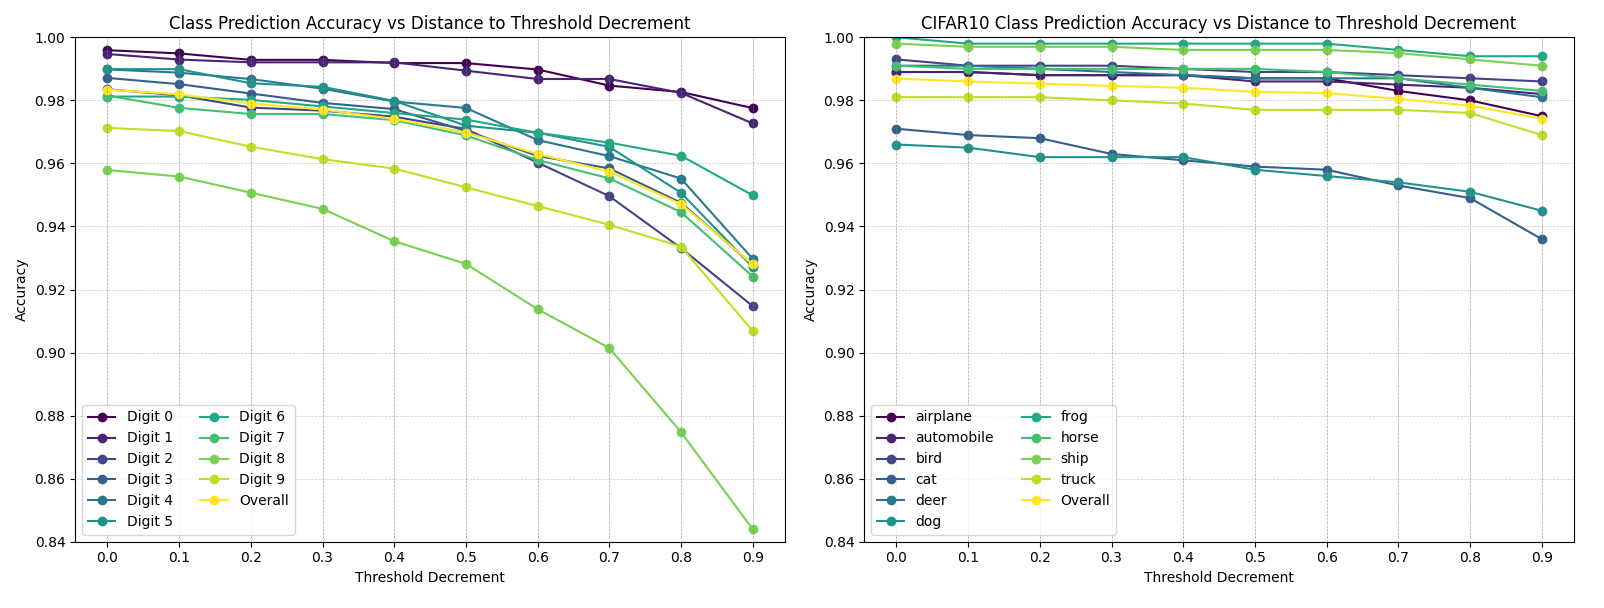
\includegraphics[width=0.99\columnwidth]{Figures/Combined_CIFAR10_MNIST_single_plot_accuracy_decrements.png}
%     \caption{Please zoom in for detail. Expected accuracy decrease as a result of threshold decrease. MNIST data is on the left, CIFAR-10 is on the right. The x axis shows the threshold decrement in factors of 0.1, that is, at 0.1 the threshold is 90\% of the original threshold while at 0.9 the threshold is 10\% of the original threshold and consequently neared to the class centroid.}
% \label{fig:Combined_CIFAR10_MNIST_single_plot_accuracy_decrements.png}
% \end{figure}

% moved to methods to spread out images
% % function call
% % plot_digit_averages(test_correct_predictions, test_incorrect_predictions, color1='lightgreen', color2='lightcoral', data="Testing Data")
% \begin{figure}[ht]
%     \centering
%     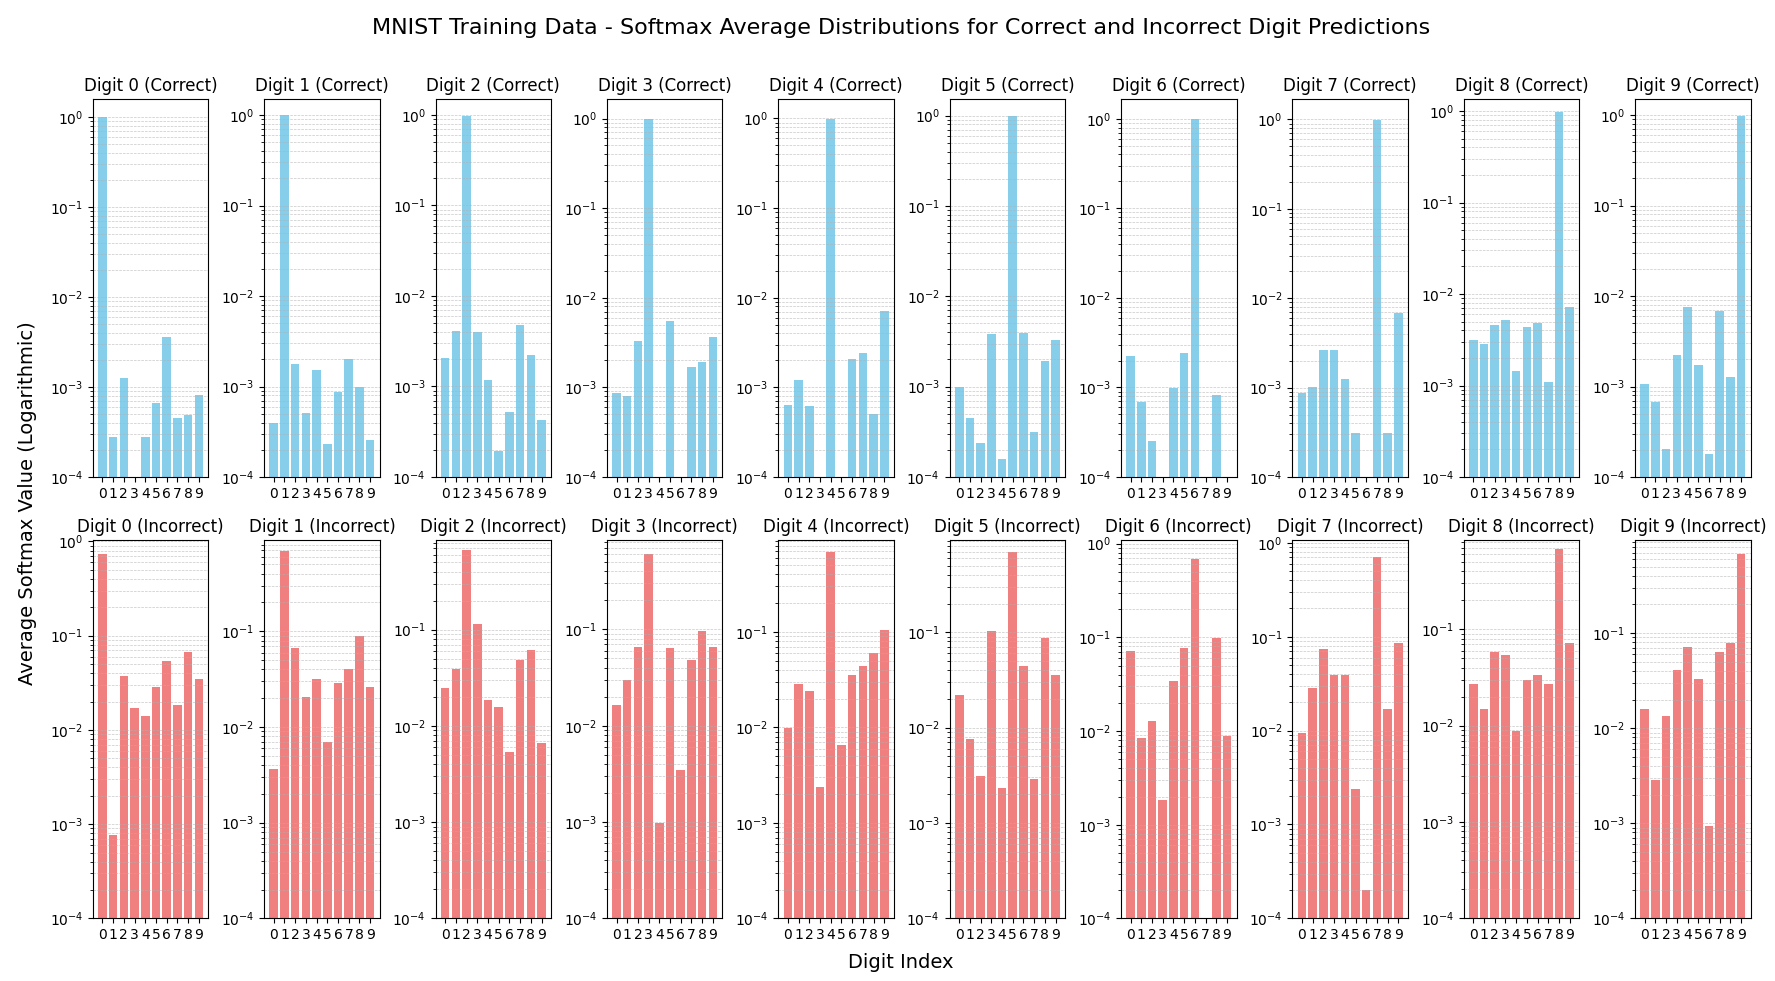
\includegraphics[width=0.99\columnwidth]{Figures/MNIST_Softmax_Averages_Training.png}
%     \caption{Please zoom in for detail. Average Softmax Probabilities for Correctly and Incorrectly Classified Digits in the MNIST Testing Dataset.}
%     \label{fig:MNIST_Softmax_Averages_Training}
% \end{figure}

% moved to appendix
% Figure \ref{fig:MNIST_Softmax_Averages_Training} shows the average softmax probabilities for each digit class (0 to 9) in the MNIST training dataset, separated into correctly classified instances (top row) and incorrectly classified instances (bottom row). The probabilities are displayed on a logarithmic scale. For correctly classified digits, the highest average probability is observed for the corresponding true digit class, indicating strong confidence in the correct predictions. In contrast, for incorrectly classified digits, the average probabilities are more evenly distributed across different digit classes, suggesting lower confidence and potential confusion between similar-looking digits.
% Figure \ref{fig:MNIST_Softmax_Averages_Testing} is the corresponding plot for the MNIST testing dataset.

% % function call
% % plot_digit_averages(test_correct_predictions, test_incorrect_predictions, color1='lightgreen', color2='lightcoral', data="Testing Data")
% \begin{figure}[ht]
%     \centering
%     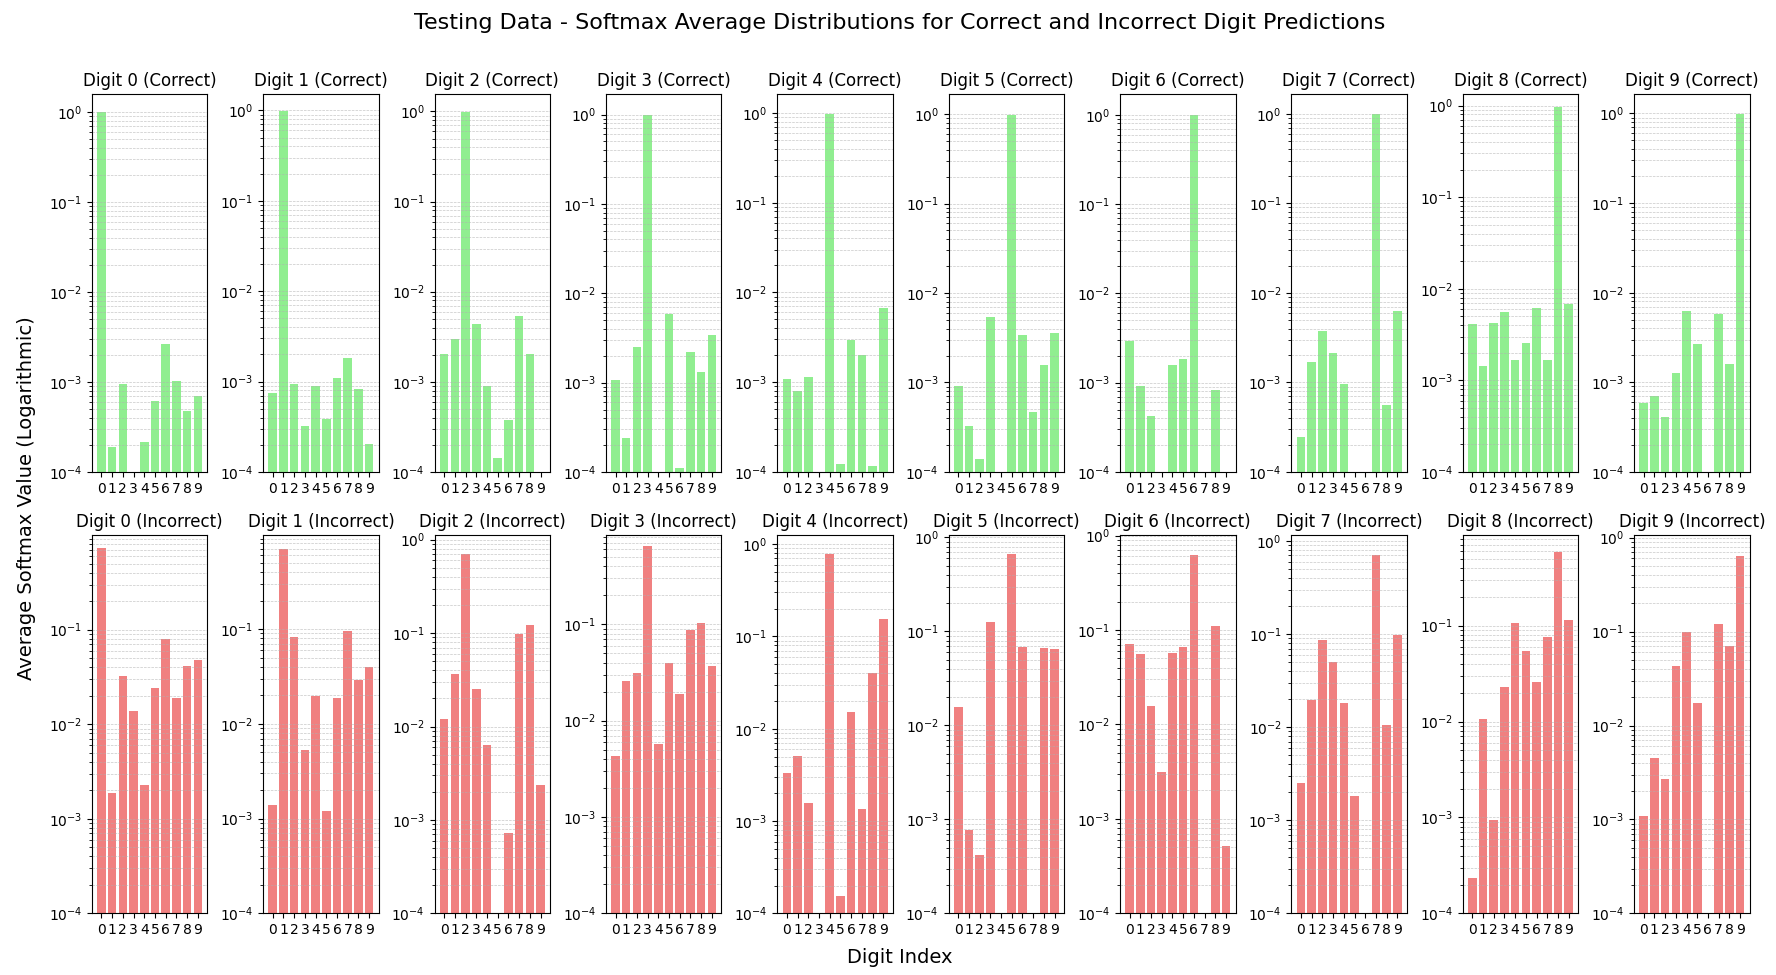
\includegraphics[width=0.99\columnwidth]{Figures/MNIST_Softmax_Averages_Testing.png}
%     \caption{Please zoom in for detail. Average Softmax Probabilities for Correctly and Incorrectly Classified Digits in the MNIST Testing Dataset.}
%     \label{fig:MNIST_Softmax_Averages_Testing}
% \end{figure}

%%%%%%%%%%%%%%%%%%%%%%%%%%%%%%%%%%%%%%%%%%%%%%%%%%%%%%%%%%%%%%%
% Average Softmax Probabilities for Correctly and Incorrectly %
% Classified Classes in the CIFAR10 dataset                   %
%%%%%%%%%%%%%%%%%%%%%%%%%%%%%%%%%%%%%%%%%%%%%%%%%%%%%%%%%%%%%%%

% Plot generated by function call
% single_plot_accuracy_decrements(accuracy_results, overall_results, labels=class_labels, dataset="CIFAR10", save=True)

% \begin{figure}[ht]
%     \centering    
%     \includegraphics[width=0.99\columnwidth]{Figures/CIFAR10_single_plot_accuracy_decrements.png}
%     \caption{Single plot Accuracy decrements}   \label{fig:CIFAR10_single_plot_accuracy_decrements}
% \end{figure}

% Function call to generate plot
% plot_centroid_distance_bars(train_correct_predictions, 
                            % train_incorrect_predictions, 
                            % labels=class_labels, 
                            % color1='lightblue', 
                            % color2='lightcoral', 
                            % data="CIFAR10 Training Data", 
                            % save=True, 
                            % filename='CIFAR10_training_plot_centroid_distance_bars.png')


% moved to methods for a better spread of images
% \begin{figure}[ht]
%     \centering
%     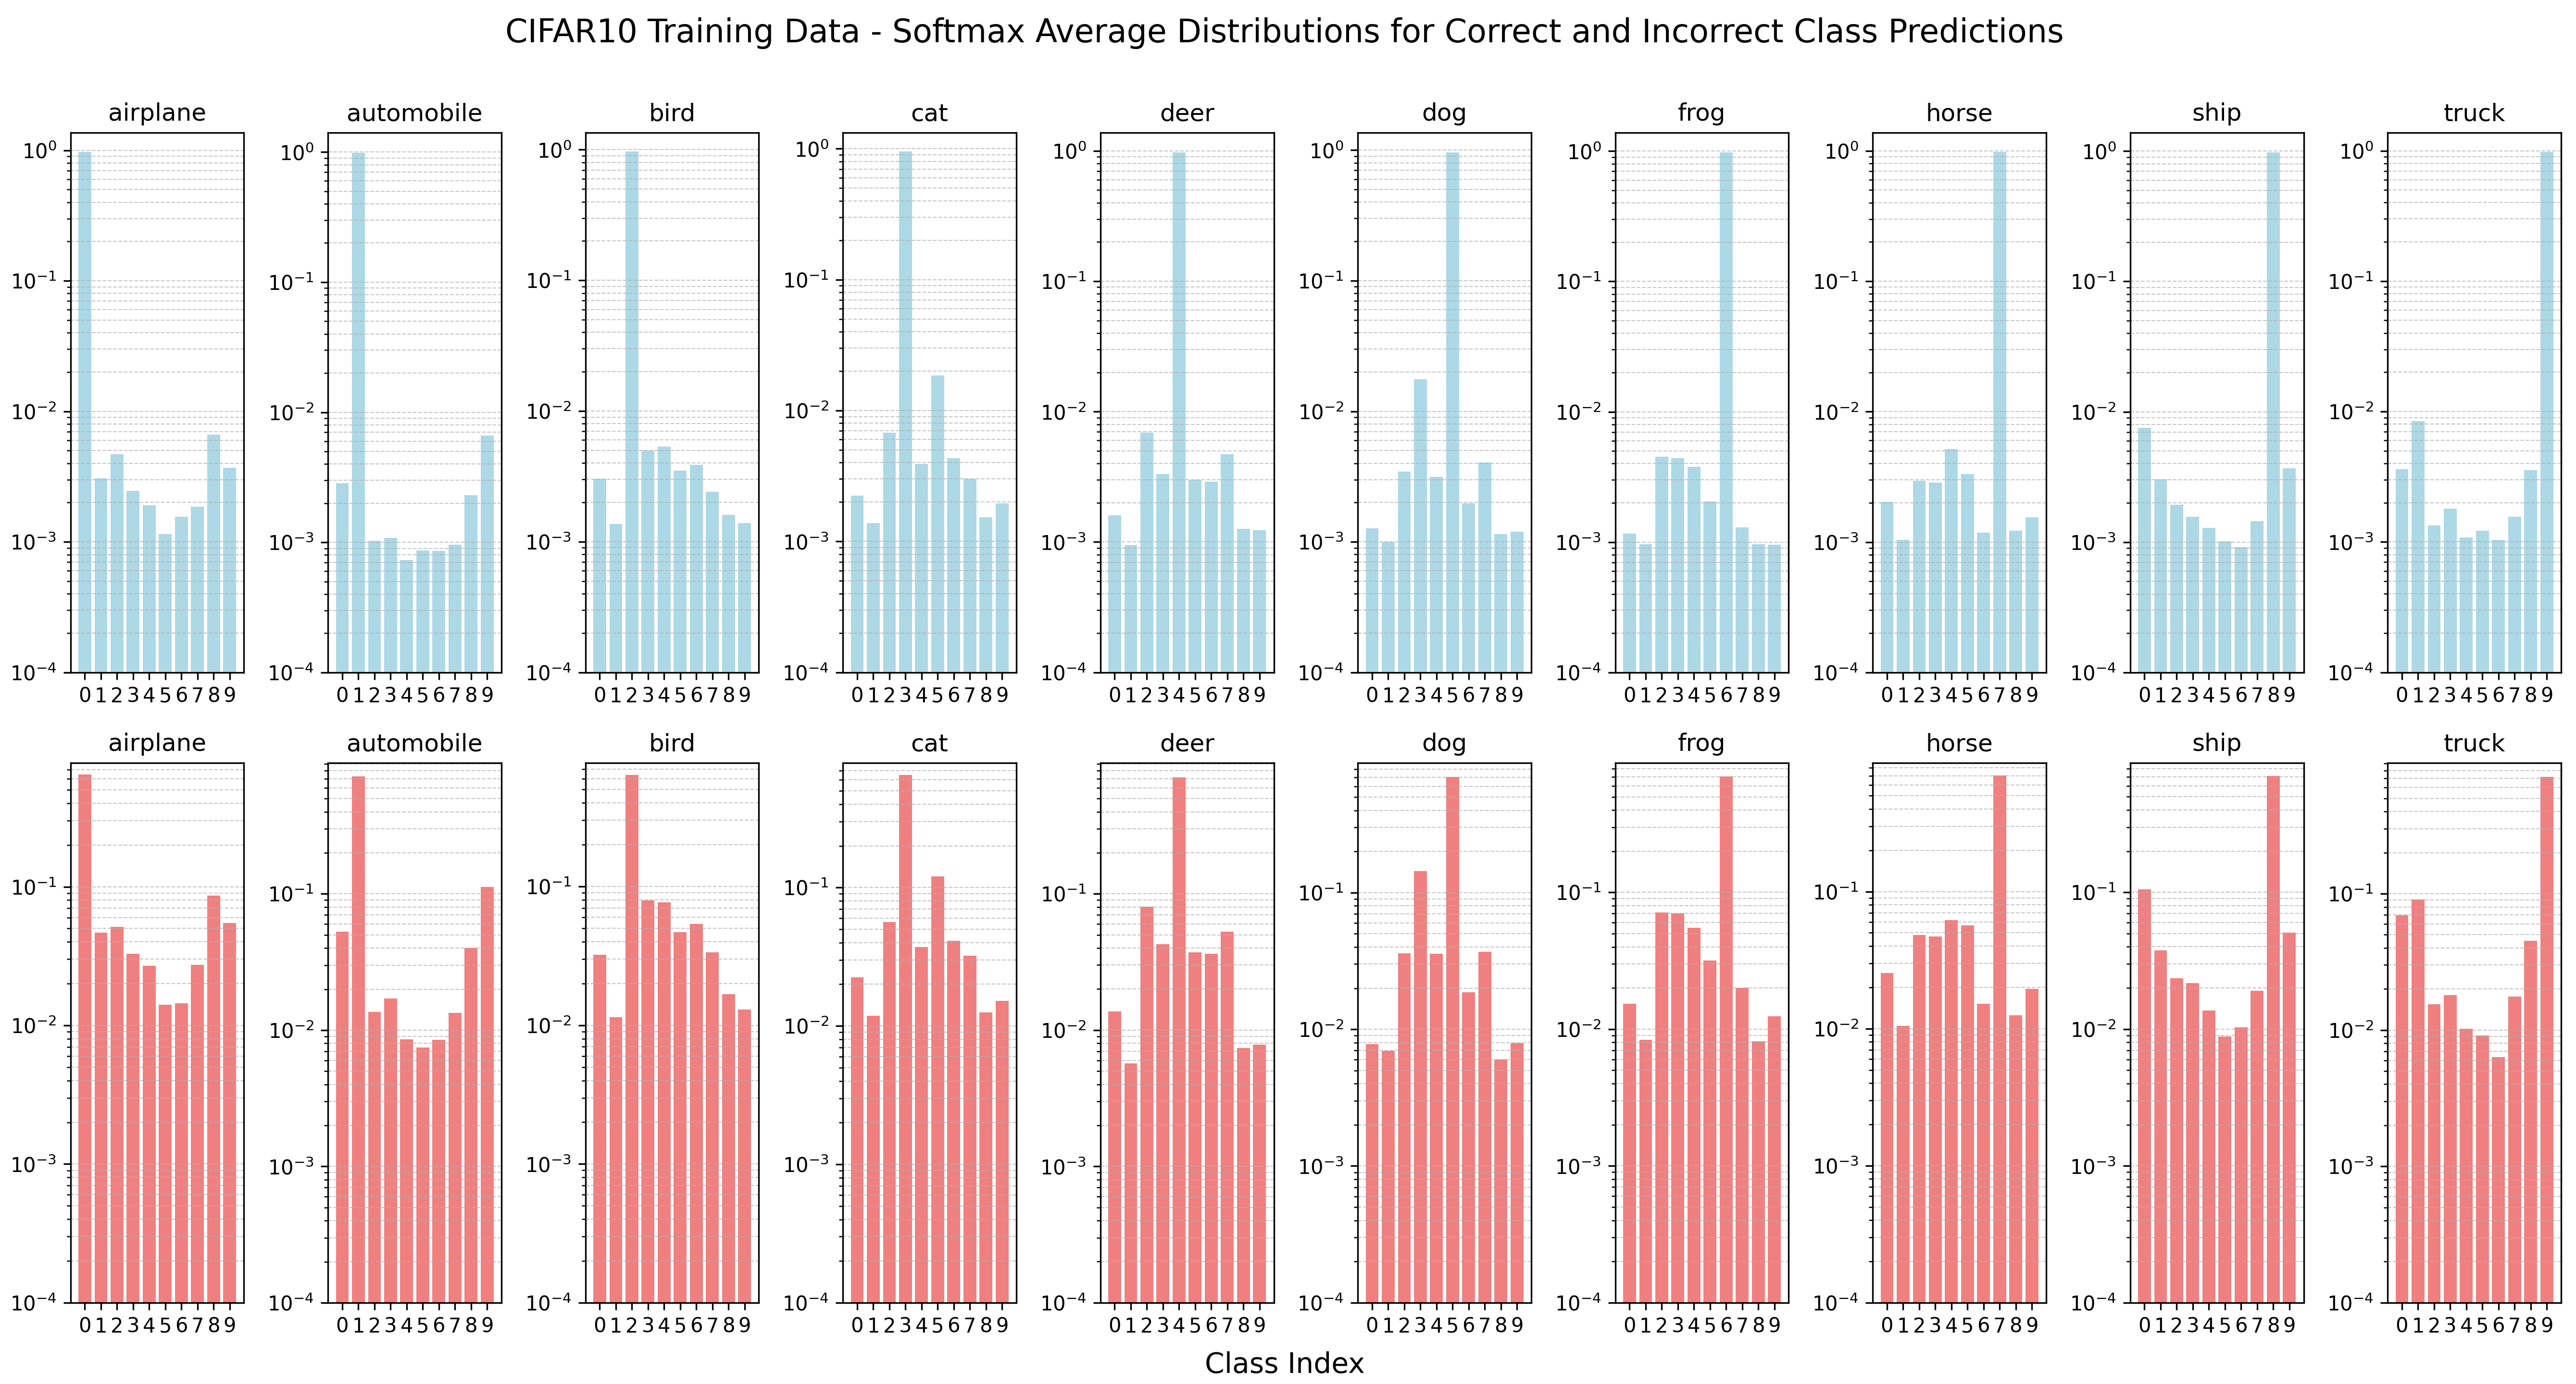
\includegraphics[width=0.95\columnwidth]{Figures/CIFAR10_training_plot_centroid_distance_bars.png}
%     \caption{Please zoom in for detail. Average Softmax Probabilities for Correctly and Incorrectly Classified Classes in the CIFAR-10 Training Dataset}
%     \label{fig:CIFAR10_training_plot_centroid_distance_bars.png}
% \end{figure}

% Function call to generate plot
% plot_centroid_distance_bars(test_correct_predictions, 
%                             test_incorrect_predictions, 
%                             labels=class_labels, 
%                             color1='lightgreen', 
%                             color2='lightcoral', 
%                             data="CIFAR10 Testing Data", 
%                             save=True, 
%                             filename='CIFAR10_testing_plot_centroid_distance_bars.png')

% Moved to Supplementary Material
% \begin{figure}[ht]
%     \centering
%     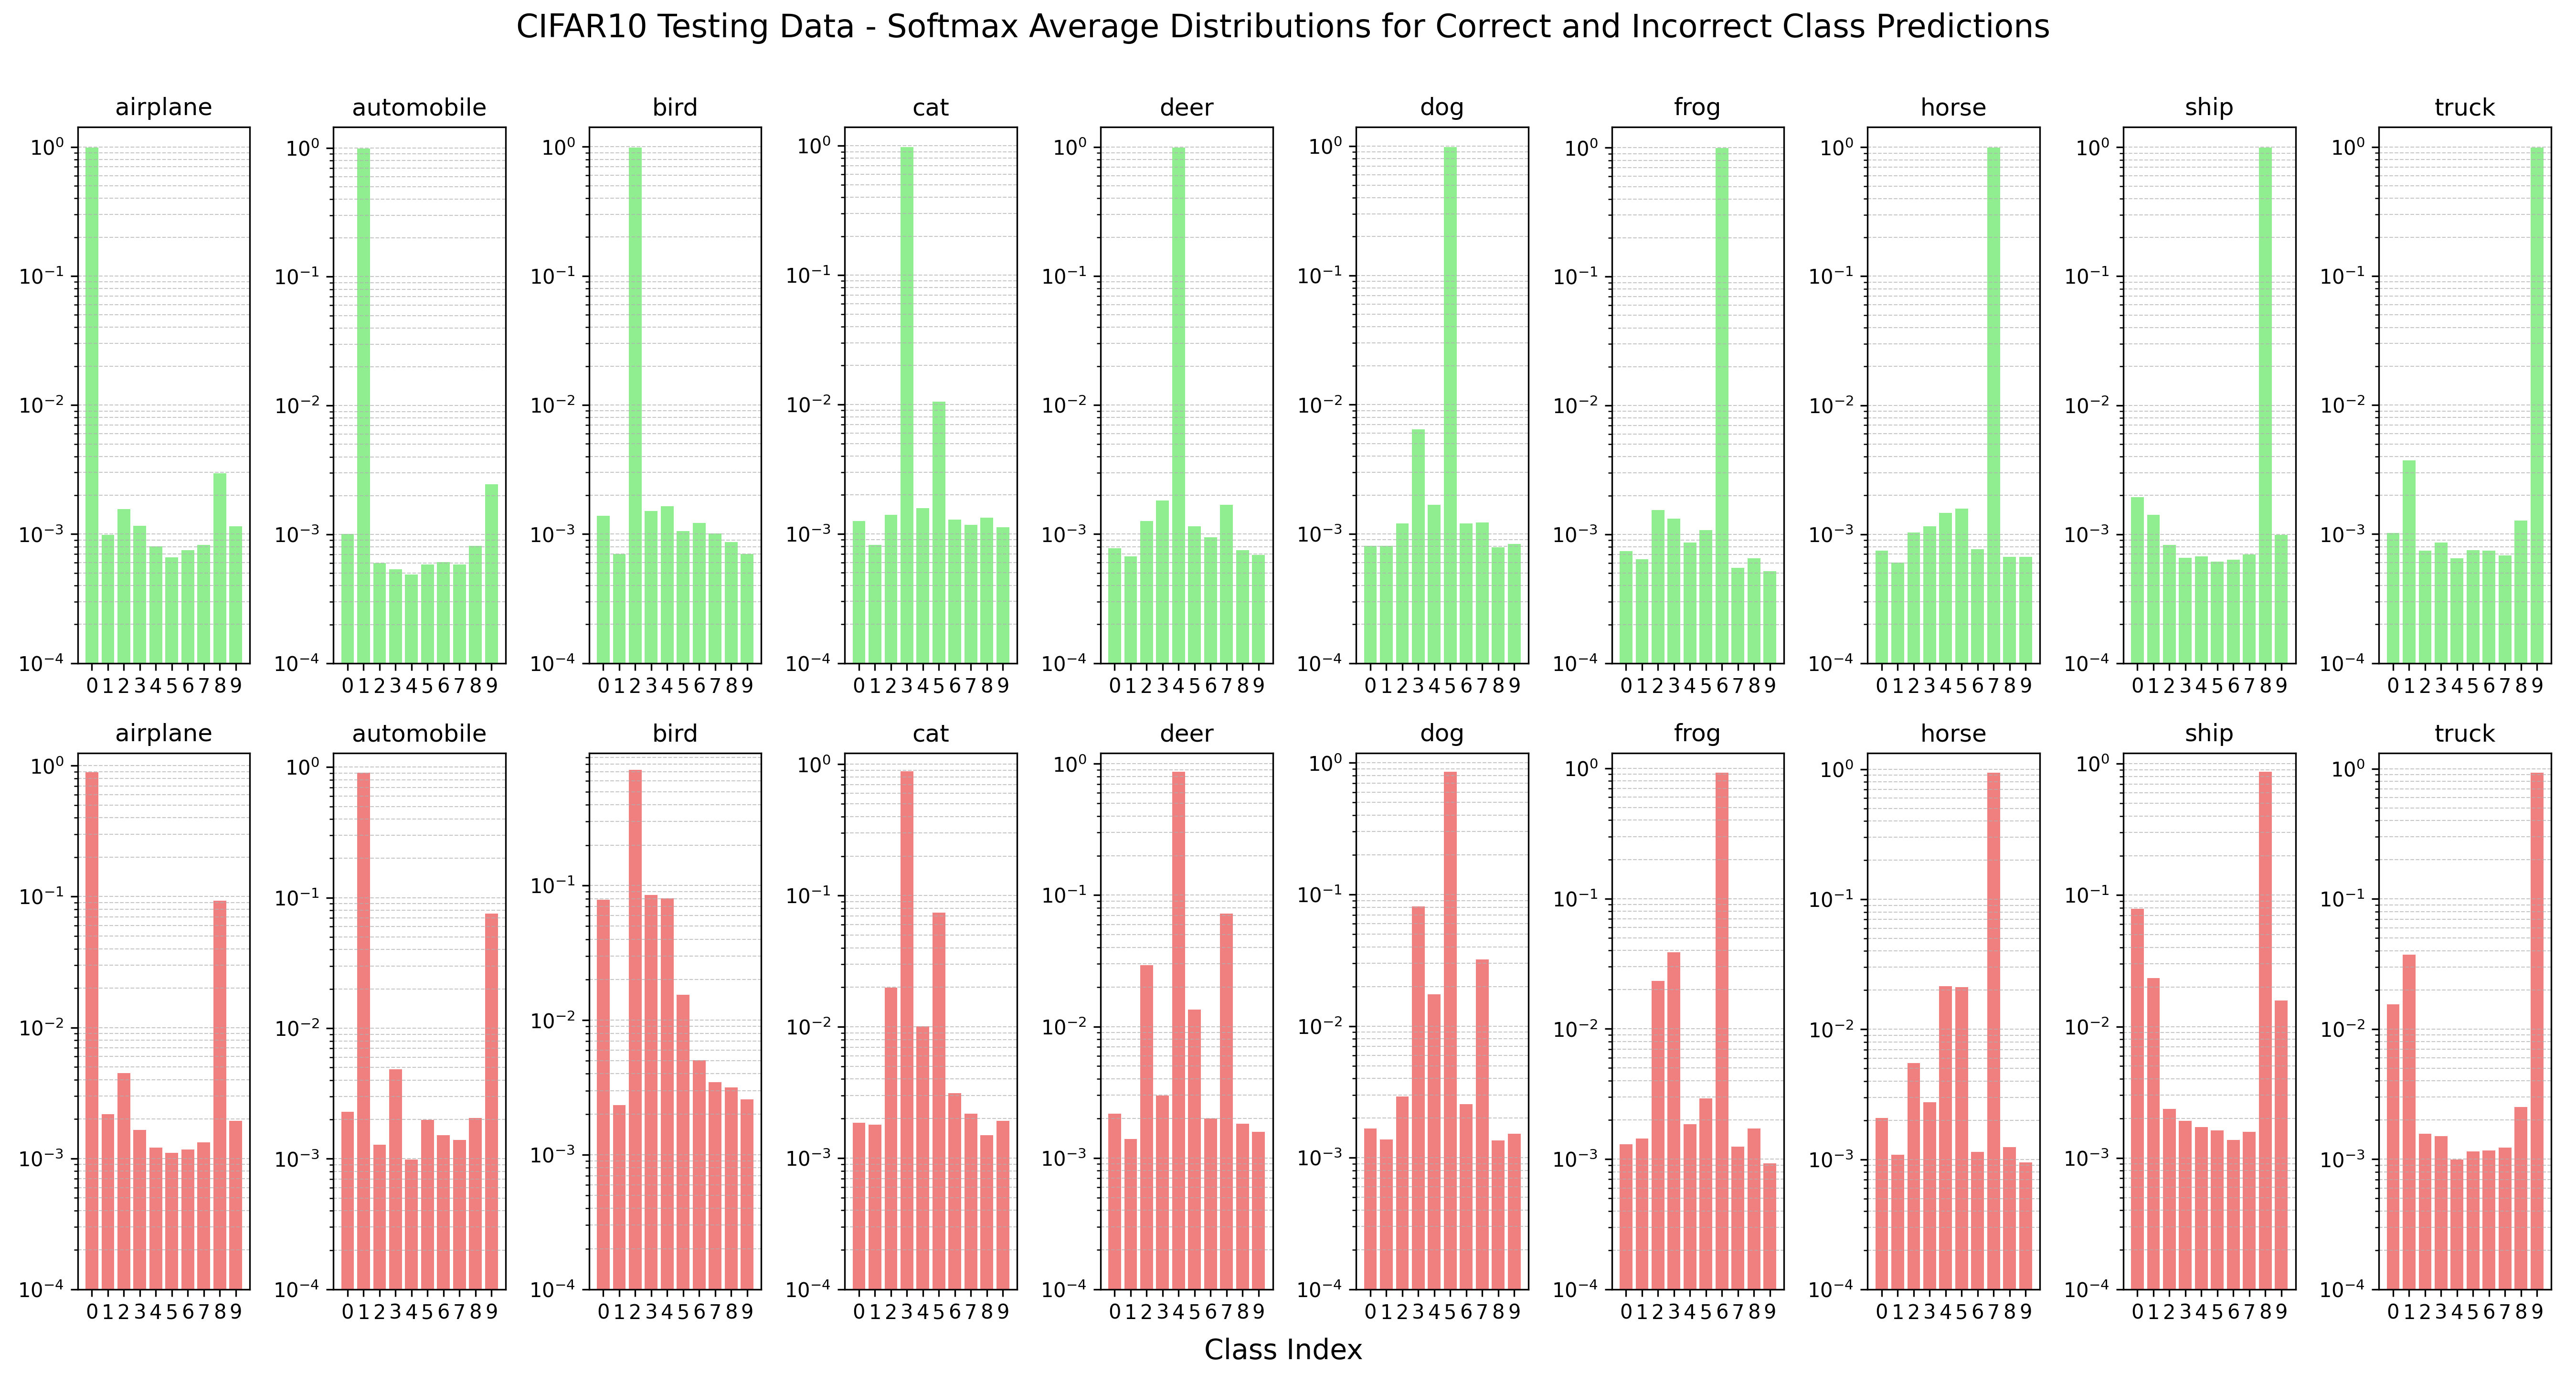
\includegraphics[width=0.95\columnwidth]{Figures/CIFAR10_testing_plot_centroid_distance_bars.png}
%     \caption{Please zoom in for detail. Average Softmax Probabilities for Correctly and Incorrectly Classified classes in the CIFAR-10 Testing Dataset}
%     \label{fig:CIFAR10_testing_plot_centroid_distance_bars.png}
% \end{figure}

% is a bar chart representing the mean softmax distances to class centroid for all correct (green) and all incorrect (red) classifications from the ViT model trained on CIFAR-10 data. 

% The softmax distribution bar charts provide a view of the model's confidence and uncertainty in its predictions. The distinct patterns observed for correct and incorrect classifications offer valuable information about the model's decision-making process.

For the CIFAR-10 we observe similar results. For correctly classified instances, the average softmax value corresponding to the true digit class is significantly higher compared to the softmax values of the other digit classes. This observation holds true across all digit classes in both the testing and training datasets. The pronounced difference in magnitudes indicates that the model assigns a high level of confidence to the correct predictions, with the predicted probability for the true class being orders of magnitude larger than the probabilities assigned to the other classes.

In contrast, for incorrectly classified instances, the average softmax values exhibit a more even distribution across the digit classes. While the softmax value for the predicted class is still relatively high, the softmax values for the other classes are notably closer in magnitude, as evident from the shorter bars on the logarithmic scale. This suggests that when the model makes an incorrect prediction, it assigns more substantial probabilities to multiple classes, indicating a higher level of uncertainty or confusion in the decision-making process.
Figures \ref{fig:CIFAR10_training_plot_centroid_distance_bars.png} and \ref{fig:CIFAR10_testing_plot_centroid_distance_bars.png} bar charts show the average softmax distributions for correct (green/blue) and incorrect (red) class predictions in both the testing and training CIFAR-10 datasets.

Comparing the testing and training datasets, we observe similar patterns in the softmax distance distributions for both correct and incorrect predictions. The consistency of these patterns suggests that our approach is consistent across datasets and models. 

The analysis of softmax distance distributions may be taken as an insight into the model's decision-making process. The difference in the softmax values between correct and incorrect predictions highlights the model's ability to discriminate between classes when it makes accurate predictions. On the other hand, the more evenly distributed softmax values for incorrect predictions suggest that the model struggles to make clear distinctions between classes in those cases, assigning considerable probabilities to multiple digits, where our proposed thresholding method may be an additional tool to help evaluate predictions in different settings.
